\chapter{Multimedia System}

\section{Introduction, Concept and Structure}
\subsection{Introduction}
The word multimedia is composed of two parts: the prefix \emph{multi} and the root \emph{media}. The prefix \emph{multi} comes from the Latin word \emph{multus}, which means ``numerous".

The root \emph{media} is the plural form of the Latin word \emph{medium}. \\

In general, \textit{medium} is a means for distribution and presentation of
information., Examples of a medium are \textit{text}, \textit{graphics}, \textit{speech} and \textit{music}.


%https://www1.udel.edu/edtech/multimedia/index.html
\noindent Multimedia is the use of a computer to present and combine text, graphics, audio, and video with links and tools that let the user navigate, interact, create, and communicate. 

This definition contains four components essential to multimedia. 
\begin{enumerate}
	\item First, there must be a computer to coordinate what we see and hear, and to interact with.
	\item Second, there must be links that connect the information. 
	\item Third, there must be navigational tools that let us traverse the web of connected information.
	\item Finally, there must be ways for us to gather, process, and communicate our own information and ideas.
\end{enumerate}

 If one of these components is missing, we do not have multimedia. For example:
 \begin{itemize}
 	\item If we have no computer to provide interactivity, we have mixed media, not multimedia. 
 	\item If there are no links to provide a sense of structure and dimension, we have a bookshelf, not multimedia. 
 	\item If there are no navigational tools to let us decide the course of action, we have a movie, not multimedia. 
 	\item If we cannot create and contribute our own ideas, we have a television, not multimedia.
 \end{itemize}

\subsection*{Multimedia Applications}
Examples of Multimedia Applications include:

\begin{multicols}{2}
\begin{itemize}
	\item World Wide Web
	\item Animation
	\item 3D Mapping
	\item Video-on-demand
	\item Interactive TV
	\item Computer Games
	\item Virtual reality
	\item Digital video editing and production systems
	\item Image processing
	\item Voice recognition
	\item Augmented reality
\end{itemize}
\end{multicols}
\subsection{Concept}
Multimedia can have many definitions these include:

\subsubsection*{A computer system perspective definition}
Multimedia means that computer information can be
represented through audio, video, and animation in addition to
traditional media (i.e., text, graphics/drawings, images).


\subsubsection*{General Definition}
Multimedia is the field concerned with the computer
controlled integration of text, graphics, drawings, still and
moving images (Video), animation, audio, and any other
media where every type of information can be represented,
stored, transmitted and processed digitally.

\subsection{Structure}
Figure {\ref{fig:multimedia-structure}} shows the main fields of multimedia systems.

%@@@@@@@@@@@@@@@@@@@@@@@@@@@@@@@@@@@@
%									@
%			FIGURE					@
%									@
%@@@@@@@@@@@@@@@@@@@@@@@@@@@@@@@@@@@@
		
\begin{figure}[H]
	\centering
	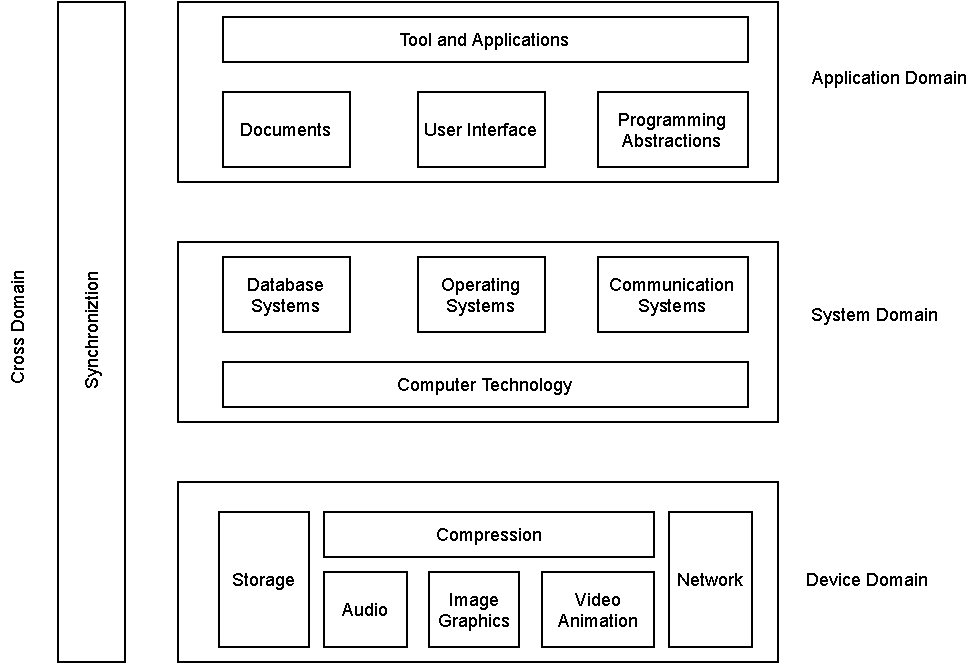
\includegraphics[width=\textwidth]{multimedia-structure}
	\caption{Main fields of multimedia systems.}\label{fig:multimedia-structure}
\end{figure}

\noindent The following areas can be distinguished:

\subsubsection*{Device Domain}
	Basic concepts for the processing of \textit{digital audio} and \textit{video} data are based
	on digital signal processing. Different methods for the	processing of \textit{image}, \textit{graphics} and \textit{animation} are included.
	
\subsubsection*{System Domain}
	The interface between the device domain and the system domain is specified
	by the \textit{computer technology}. To utilize the device domain, several system services are needed. Basically, three services exist. These services are mostly implemented in software:
		\begin{itemize}
			\item The \textit{operating system} serves as an interface between computer hardware/system software and all other software components.
			
			\item The \textit{database system }allows structured access to data and a management of large databases.
			
			\item The \textit{communication system} is responsible for data transmission according to the timing and reliability requirements of the networked multimedia application.
		\end{itemize}
	
	
\subsubsection*{Application Domain}
	
	The services of the system domain are offered to the application domain through proper programming abstractions.
	
	Another application domain is \textit{document handling}. A document consists of a set of structured information, represented in different media, and generated or recorded at the time of presentation.
	
	Many functions of document handling and other applications are accessible and presented to the user through a \textit{user interface}.
	
\subsubsection*{Cross Domain}
Some aspects, such as synchronization aspects, are difficult to locate in one or two components or domains. The reason is that \textit{synchronization}, being the temporal relationship among various media, relates to many components across all domains.


\section{Media Aspect Properties}
Media can be classified with respect to different criteria as follows:
\begin{multicols}{2}
	\begin{itemize}
	\item perception media 
	\item representation media
	\item presentation media
	\item storage media
	\item transmission media
	\item information exchange media
	\end{itemize}
\end{multicols}


\subsection{Perception Media}
Perception media refers to the nature of information perceived by humans. The question to ask here is: \emph{How do humans perceive information}? The answer is that the perception of information occurs mostly through seeing or hearing the information.

We distinguish primarily between what we see and what we hear. 
\begin{itemize}
	\item \textit{Auditory media} include music, sound, and voice. 
	\item \textit{Visual media} include text, graphics, and still and moving pictures.
\end{itemize}


\subsection{Representation Media}
The term representation media refers to how information is represented internally
to the computer. The question to ask here
is: \emph{How is information encoded in the computer?} The
answer is that various formats are used to represent media information in a computer. There are several options:

\begin{itemize}
\item A text character is coded in \gls{ascii} or \gls{ebcdic} code.
\item Graphics are encoded using \gls{gks} graphics standard.
\item An audio stream can be represented using \gls{pcm}
\item An image is in \gls{jpeg} format.
\item A combined audio-video sequence is stored in the computer in various TV standards (e.g., \gls{pal}, or \gls{ntsc}, or in \gls{mpeg} format).
\end{itemize}

\subsection{Presentation Media}
Presentation media refers to the physical means used by systems to reproduce information for humans. The question to ask here is: \emph{Which medium is used to output information
from the computer or input in the computer?}

We distinguish primarily between output and input media:
\begin{itemize}
	\item \textit{output media}: paper, computer monitors, and loudspeakers, etc.
	\item \textit{input media}: keyboards, cameras, and microphones, etc.
\end{itemize}


\subsection{Storage Media}
Storage media refers to various physical
means for storing computer data, such as magnetic tapes, magnetic disks, or digital
optical disks. However, data storage is not limited to the components available in a
computer, which means that paper is also a storage medium. The question to
ask here is: \emph{Where is information stored?} Example of storage media includes: \textit{Hard disk}, \textit{\gls{cd}}, \textit{\gls{usb} flash drive}\footnote{\textnp{बाेलीचालीकाे भाषामा पेन ड्राइभ (pen drive) पनि भनिन्छ}}, etc. 

\subsection{Transmission Media}
Transmission media refers to the physical media. The question to ask here is:
\emph{Which medium is used to transmit data?} The answer is that information is transmitted over networks, cables such as fiber or coaxial as well as free airspace transmission for wireless transmission.

\subsection{Information Exchange Media}
Information exchange media includes all data media used to transport information,
e.g., all storage and transmission media. The question to ask here is: \emph{Which data
medium is used to exchange information between different locations?}

For example, information can be exchanged by storing it on a removable medium
and transporting the medium from one location to another. These storage media include
microfilms, paper, and USBs, etc.

\section{Definition of Multimedia System}
A Multimedia System is a system capable of processing multimedia data and applications. A Multimedia System is characterized by the processing, storage, generation, manipulation and interpretation of Multimedia
information.


Characteristics of Multimedia System:

\begin{itemize}
	\item They must be computer-controlled.
	\item They are integrated.
	\item They must support media independence.
	\item And lastly, they need to handle discrete and continuous media.
\end{itemize}

\subsection{Discrete and Continuous Media}
If the application uses both discrete and continuous media then it is called multimedia. This means that a multimedia application should process at least one discrete and one continuous medium. A word processor with embedded graphics is not a multimedia application.

\subsection{Independent Media}
Media should not be tightly coupled together. They must be independent for example, digital audio and computer available text can be combined for the purpose of presentation. 

\subsection{Computer-Controlled Systems}
The independence of media creates a way to combine media for presentation. For this purpose, the computer is the ideal tool. The system can be optionally programmed by a programmer. The simple video recording and playback of media is a system such as video recorder is not sufficient to meet the requirements for computer controlled systems. 

\subsection{Integration}
Computer-controlled independent media streams can be integrated to form a global system so that, together, they provide a certain function. A word processor
that supports text, spreadsheets, and graphics does not meet the integration criterion
unless it allows program-supported references between the data. 

\section{Traditional Data Stream Characteristics}
Distributed networked multimedia systems transmit both discrete and continuous
media streams. In a digital system, information is split
into units (packets) before it is transmitted. These packets are sent by one system component (the \textit{source}) and received by another one (the \textit{sink}). Source and sink can reside on different computers. A data stream consists of a (temporal) sequence of packets. 

Packets can carry information from continuous and discrete media. 
\begin{itemize}
	\item Continuous medium: \textit{transmission of voice in a telephone system}
	\item Discrete medium : \textit{transmission of text file}
\end{itemize}


When we transmit information originating from various media, we obtain data
streams that have very different characteristics. The attributes 
\begin{multicols}{3}
\begin{enumerate}[label=\alph*)]
	\item asynchronous
	\item synchronous and 
	\item isochronous
\end{enumerate}
\end{multicols}


 are traditionally used in the field of telecommunications to describe the characteristics of a data transmission.


\subsection{Asynchronous Transmission Mode}
A communication is called asynchronous if a
sender and receiver do not need to coordinate before data can be transmitted. 
\begin{itemize}
	\item In asynchronous transmission, the transmission may start at any given instant.
	\item The bit synchronization that determines the start of each bit is provided by two independent clocks on both sender and receiver.
	\item Example: ASCII terminals attached to host computers. Whenever a character is pressed, a sequence of bits is generated and sent to the computer interface along with character.
	\item A special signal called \textit{start} signal precedes the information bits.
	\item Another special signal called \textit{stop} signal follows the last information bit.
\end{itemize}

\subsection{Synchronous Transmission Mode}
The synchronous transmission mode defines a maximum end-to-end delay for each packet of a data stream. This upper bound will never be violated.

In synchronous transmission, transmission begins when the clock signal is matched with the receiver.


\subsection{Isochronous Transmission Mode}
The isochronous transmission mode defines, besides a maximum end-to-end delay for each packet of a data stream, a minimum end-to-end delay.
\begin{itemize}
	\item This mode is a form of data transmission in which individual characters are only separated by a whole number of bit-length intervals. 
	\item For example, an end-to-end network connection is said to be isochronous if the bit rate over the connection is guaranteed and if the value of the delay \textit{jitter} is also guaranteed and small.
\end{itemize}

\section{Data Stream Characteristics For Continuous Media}
Following are the data stream characteristics that relate to any audio/video data transfer in a multimedia system (multimedia data streams).
\begin{itemize}
	\item The time interval between a complete transmission of consecutive packets.
	\item Variation of consecutive packet amount.
	\item Contiguous packets.
\end{itemize}

\subsection{The Time Interval Between a Complete Transmission of Consecutive Packets}
The first property of data streams relates to the time intervals between fully completed transmissions of consecutive information units or packets. Based on the moment
in which the packets become ready, we distinguish between the following variants:

\subsubsection{Strongly Periodic Data Stream}
\begin{itemize}
	\item When the time interval between neighboring packets is constant, then this data
	stream is called a \textit{strongly periodic} data stream.
	\item This also means that there is minimal jitter—ideally zero.
	\item Example: PCM-encoded voice in telephone systems.
\end{itemize}

 Figure {\ref{fig:strongly-periodic}} illustrates strongly periodic data stream.

%@@@@@@@@@@@@@@@@@@@@@@@@@@@@@@@@@@@@
%									@
%			FIGURE					@
%									@
%@@@@@@@@@@@@@@@@@@@@@@@@@@@@@@@@@@@@
\begin{figure}[ht]
\centering
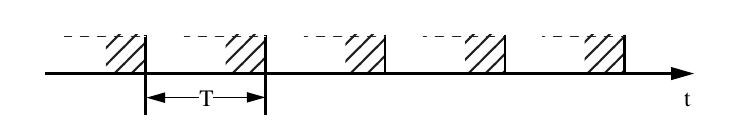
\includegraphics[width=\textwidth]{strongly-periodic}
\caption[Strongly periodic data stream]{Strongly periodic data stream; time intervals have the same duration between consecutive packets.}\label{fig:strongly-periodic}
\end{figure}

\subsubsection{Weakly Periodic Data Stream}
The duration of the time intervals between neighboring packets is often described
as a \textit{function with finite period duration}. However, this time interval is not constant between neighboring packets. The data stream is called \textit{weakly periodic}. The case is shown in Figure {\ref{fig:weakly-periodic}}.

%@@@@@@@@@@@@@@@@@@@@@@@@@@@@@@@@@@@@
%									@
%			FIGURE					@
%									@
%@@@@@@@@@@@@@@@@@@@@@@@@@@@@@@@@@@@@
\begin{figure}[ht]
	\centering
	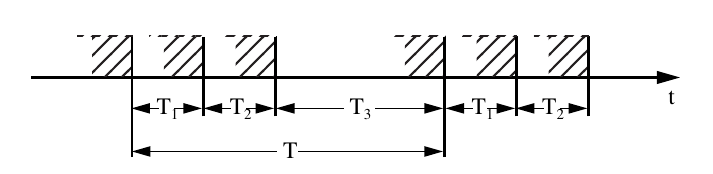
\includegraphics[width=\textwidth]{weakly-periodic}
	\caption[Weakly periodic data stream]{Weakly periodic data stream; time intervals between consecutive packets are periodic.}\label{fig:weakly-periodic}
\end{figure}

\subsubsection{Aperiodic Data Stream}
All other transmission options are called aperiodic data streams  (excluding strongly and weakly data stream), which relates to
the sequence of time interval duration, as shown in Figure {\ref{fig:aperiodic}}.

%@@@@@@@@@@@@@@@@@@@@@@@@@@@@@@@@@@@@
%									@
%			FIGURE					@
%									@
%@@@@@@@@@@@@@@@@@@@@@@@@@@@@@@@@@@@@
\begin{figure}[hb!]
	\centering
	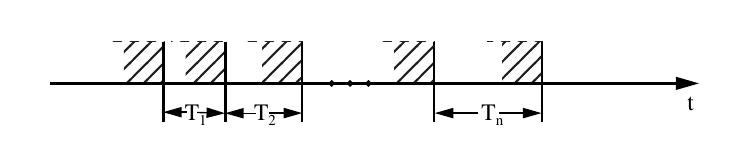
\includegraphics[width=\textwidth]{aperiodic}
	\caption[Aperiodic data stream]{Aperiodic data stream; the time interval sequence is neither constant nor weakly periodic.}\label{fig:aperiodic}
\end{figure}

An example of an aperiodic data stream is a multimedia conference application
with a common screen window. Often, the status (left button pressed) and the current
coordinates of the mouse moved by another user have to be transmitted to other participants.

\subsection{Variation of Consecutive Packet Amount}
A second characteristic to qualify data streams concerns how the data quantity of
consecutive information units or packets varies.

\subsubsection{Strongly Regular Data Stream}
\begin{itemize}
	\item If the quantity of data remains constant during the entire lifetime of a data stream, then we speak of a \textit{strongly regular data stream}.
	\item This characteristic is typical for an uncompressed digital audio-video
	stream.
	\item Examples are a the video stream taken from a camera in uncompressed form and the audio stream from an audio \gls{cd}.
\end{itemize}
 Figure {\ref{fig:strongly-regular-data-stream}} shows strongly regular data stream.  
	
%@@@@@@@@@@@@@@@@@@@@@@@@@@@@@@@@@@@@
%									@
%			FIGURE					@
%									@
%@@@@@@@@@@@@@@@@@@@@@@@@@@@@@@@@@@@@
	\begin{figure}[hb]
		\centering
		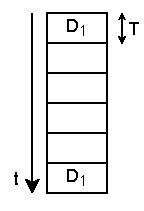
\includegraphics[width=0.3\textwidth]{strongly-regular-data}
		\caption[Strongly regular data stream]{Strongly regular data stream; the data quantity is constant in all packets.}
		\label{fig:strongly-regular-data-stream}
	\end{figure}

\subsubsection{Weakly Regular Data Stream}
\begin{itemize}
	\item If the quantity of data varies periodically (over time), then this is a \textit{weakly regular data stream}. 
	\item Example: Compressed video stream which uses a compression method such as \gls{mpeg}.
\end{itemize}


Figure {\ref{fig:weakly-regular-data-stream}} shows an example of weakly regular data stream.
	
%@@@@@@@@@@@@@@@@@@@@@@@@@@@@@@@@@@@@
%									@
%			FIGURE					@
%									@
%@@@@@@@@@@@@@@@@@@@@@@@@@@@@@@@@@@@@
	\begin{figure}[ht]
		\centering
		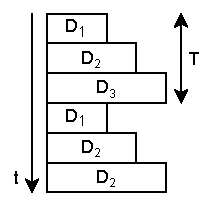
\includegraphics[width=0.3\textwidth]{weakly-regular-data}
		\caption[Weakly regular data stream]{Weakly regular data stream; the packets’ data stream varies periodically.}\label{fig:weakly-regular-data-stream}
	\end{figure}
	
\subsubsection{Irregular Data Stream}
Data streams are called irregular when the data quantity is neither constant, nor
changing by a periodic function (see Figure {\ref{fig:irregular-data-stream}}). This data stream is more difficult to transmit and process compared to the variants described earlier.

%@@@@@@@@@@@@@@@@@@@@@@@@@@@@@@@@@@@@
%									@
%			FIGURE					@
%									@
%@@@@@@@@@@@@@@@@@@@@@@@@@@@@@@@@@@@@
\begin{figure}[hb]
	\centering
	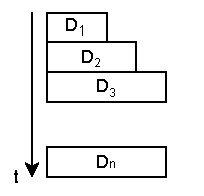
\includegraphics[width=0.3\textwidth]{irregular-data-stream}
	\caption[Irregular data stream]{Irregular data stream; the packets’ data quantity is not constant and does not vary periodically.}\label{fig:irregular-data-stream}
\end{figure}


When applying a compression method that creates a data stream with a variable
bit rate, the size of the single information units (each derived from a single image) is determined from the image content that has changed in respect to the previous image.
The size of the resulting information units normally depends on the video sequence and
the data stream is irregular.

\subsection{Contiguous Packets}
The third qualification characteristic concerns the continuity or the relationship
between consecutive packets. Are packets transmitted progressively, or is there a gap
between packets?  This can be seen as utilization of a certain system resource, such as a network.

\subsubsection{Interrelated/Continuous Data Stream}
\begin{itemize}
	\item All packets are transmitted one after the other without gaps in between.
	\item Additional information to identify user data is included, e.\ g.\, error detection codes.
	\item In this case specific resource is utilized at 100\%.
	\item Allows maximum throughput and achieves optimum utilization of a resource.
\end{itemize}
Figure {\ref{fig:interrelated-data-stream}} shows an interrelated/continuous information transfer.

%@@@@@@@@@@@@@@@@@@@@@@@@@@@@@@@@@@@@
%									@
%			FIGURE					@
%									@
%@@@@@@@@@@@@@@@@@@@@@@@@@@@@@@@@@@@@
\begin{figure}[hb]
	\centering
	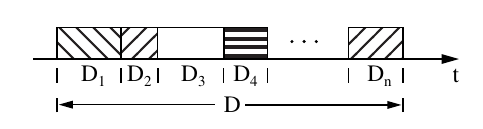
\includegraphics[width=0.8\textwidth]{interrelated-data-stream}
	\caption[Interrelated data stream.]{Interrelated data stream; packets are transmitted without gaps in between.}\label{fig:interrelated-data-stream}
\end{figure}

\subsubsection{Non-interrelated/Discrete Data Stream}
\begin{itemize}
	\item The transmission of an interrelated data stream over a higher-capacity channel
	causes gaps between packets.
	\item Each data stream that includes gaps between its information units is called a \textit{non-interrelated/discrete} data stream.
	\item It is not important if gaps exist among all packets or if the duration of gaps varies.
\end{itemize}
 Figure {\ref{fig:noninterrelated-data-stream}} shows an example of non-interrelated data stream.
 
%@@@@@@@@@@@@@@@@@@@@@@@@@@@@@@@@@@@@
%									@
%			FIGURE					@
%									@
%@@@@@@@@@@@@@@@@@@@@@@@@@@@@@@@@@@@@
\begin{figure}[ht!]
	\centering
	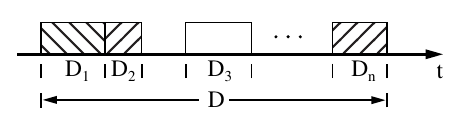
\includegraphics[width=0.8\textwidth]{non-interrelated-data-stream}
	\caption[Non-interrelated data stream.]{Non-interrelated data stream; there are gaps between packets.}\label{fig:noninterrelated-data-stream}
\end{figure}


\section{Information Units}
Continuous (time-dependent) media consist of a (temporal) sequence of information units. Such an information unit is called a \gls{ldu}, which is based on \gls{pdu}. An \gls{ldu}’s information quantity and data quantities can have different meanings:

%@@@@@@@@@@@@@@@@@@@@@@@@@@@@@@@@@@@@
%									@
%			FIGURE					@
%									@
%@@@@@@@@@@@@@@@@@@@@@@@@@@@@@@@@@@@@
\begin{figure}[hb!]                                                                    
	\centering
	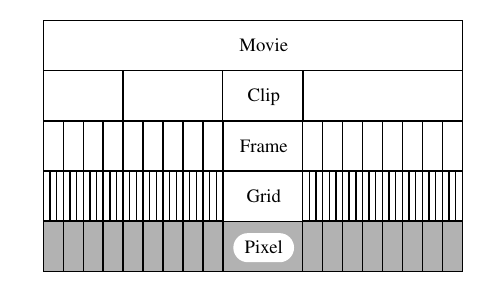
\includegraphics[width=\textwidth]{information-units}
	\caption[Information units.]{Granularity of a motion video sequence showing its \gls{ldu}s}\label{fig:information-units}
\end{figure}

\begin{itemize}
	\item In Figure {\ref{fig:information-units}}, we see that the uncompressed video sequence consists of single \textit{clips}, each representing a \textit{scene}.
	\item Each of these scenes consists of a sequence of single \textit{images}.
	\item An image can be divided, for example \(16\times16\) groups of \textit{pixels}.
	\item In turn, each pixel contains a \textit{luminance} value and a \textit{chrominance} value.
\end{itemize}

This means that a single image is not the only possible LDU in a motion video sequence. A scene or a pixel can also be an \gls{ldu}. The redundancies in single image sequences of an \gls{mpeg}-encoded video stream can be used to reduce the data quantity by applying an interframe compression method. In this case, the
smallest self-sufficient meaningful units are single-image sequences.



A phenomenon called granularity characterizes the hierarchical decomposition of
an audio or video stream in its components. This example uses a motion video to generally describe extensive information units. 

We distinguish between closed and open \gls{ldu}s:
\begin{itemize}
	\item \textit{Closed \gls{ldu}s} have a well-defined duration. They are normally stored sequences. Example: data stream of audio samples in the computer.
		
	\item In \textit{Open \gls{ldu}s}, the data stream’s duration is not known in advance. Such a data stream is delivered to the computer by a camera, a microphone, or a similar device.
\end{itemize}


\newpage\thispagestyle{empty}
